

\chapter{Object detection}

\begin{introduction}
In this chapter we will present one of the techniques used to detect archaeological sites, object detection.
\end{introduction}

One of the challenges of artificial intelligence is image classification, i.e. identifying which class the content of the image belongs to. However, another more challenging problem is object detection, i.e. identifying where the object is within the image.

One of the first algorithms to be made for this purpose, is the RCNN, this algorithm consists in generating about 2000 regions of interest in the image with the selective search algorithm, and then make image classification in these 2000 proposed regions, using a CNN. Although this algorithm can give good results, one of the problems is that it is very slow, giving an average of 47 seconds per image. 

Later, two other algorithms were created, the Fast RCNN and the Faster RCNN, showing improvements, the latter being able to process an image in mere seconds.

Later in 2016, a paper was published of a model, with an architecture called You Only Look Once (YOLO), which has since had several versions, the latest being YOLOv8.
YOLO is considered state of the art when it comes to object detection.

Of the methods presented in the previous chapter, the one chosen was the image creation from the information provided by the LIDAR, and 4 LRM images were created. However the creation of these images is not part of this dissertation, having been provided by another group belonging to the ODYSSEY project, as well the annotations.

Having the LRM images and the respective annotations, the objective of this chapter is to use YOLOv7 to discover archaeological sites.

Esta parte nao esta muito bem!!!!!!!!!!!!!!!!!!!!!!!!!!

The annotations are provided as csv files, however each annotation is saved in WKT (Well-known text) format.

The objects of study will be tumuli and hillforts, there are a total of 270 tumuli and 163 hillforts, however these annotations are not the result of a deep analysis of the terrain, thus creating the possibility that there are more objects
to detect.

After creating the dataset, the YOLOv7 model was trained, as well as a
machine learning model, with the raw data, in an attempt to eliminate false positives resulting from YOLOv7.

The two objects under study, are quite different, the tumuli on the one hand, have a very regular shape, uniform and of very equal size, on the other hand, the hillforts already have a very non-uniform shape and various sizes.

Finally, the training results of the trained models will be analyzed.


\section{YOLO}
While the 3 methods presented, RCNN, Fast RCNN, and Faster RCNN, all of them run the image several times through the algorithm, YOLO comes with a different idea, the image only passes through the model once.

For this, the image is divided into a grid\cite{yolodeepdive} with several cells, the image is then processed by the model, generating a two dimensional tensor, with the number of rows equal to the number of cells, and columns equal to 5 + number of object classes. In other words, each cell has a vector associated with the probability of having an object with the central point of the bounding box inside it.

y = [pc, cx, cy, w, h, c0, c1, c2,...].

\begin{itemize}
    \item pc is the probability of being the identified object.
    \item cx and cy is the center point of the bounding box.
    \item w and h are the width and height of the bounding box.
    \item c0, c1, c2, ... indicates which class the detection belongs to.
\end{itemize}

However, this approach presents a problem, because for the same object several bounding boxes can appear, for this the algorithm uses a function called NMS (Non Maximum Suppression).

\subsubsection{Non Maximum Suppression}
Non Maximum Suppression \cite{nonmaxsurpression} is a method that selects a region from a series of overlapping regions. First it discards all proposed regions with a probability below a certain threshold. For the remaining ones it chooses the region with the highest probability and discards all the others that have an IoU higher than a certain threshold.
IoU is the intersection over union, that is the area of the region in question divided by the union of the areas of all the regions that overlap with that same region.

IoU is the intersection over union, this means the area of intersection of the overlapping regions to be divided by the area of the union.


\subsection{Training}
Neural network training is a fundamental step in deep learning, it is in this phase that the network will "learn" how to perform the task at hand, this can range from image classification, object detection, language processing and many other applications.

To do this it is common to divide the dataset into 3 parts, training, validation and testing. During training the net goes through several iterations called epochs, where it learns to make predictions by adjusting its internal parameters based on the provided training data.
The training process consists of feeding the neural net with batches of training data.
A batch is a subset of the training data set, instead of feeding the entire training data set to the neural net, it is divided into batches, making the process more computationally efficient, and also allowing the weights of the neural net to be adjusted more often, since they are updated at the end of each batch.

At the end of the batch processing, the error is calculated relative to the predictions made by the model and the labels. This error is usually measured by a loss function, such as cross entropy or least squares error. After the error is calculated, the optimization algorithm, such as SGD or Adam, is used to adjust the weights of the neural network in a direction that minimizes the error. To do this a back propagation function is used, where the error is propagated from the output layer to the input layer, allowing each neuron to update its weights in order to contribute to the reduction of the total error.

At the end of each epoch, a validation of the model is then performed with the validation set, that is, the data from the validation set is used to evaluate the performance of the trained model up to that point. Model validation is crucial for monitoring the generalization ability of the model over the course of training. It provides information on how the model is performing on data not used during training, and helps identify problems such as overfitting. Overfitting occurs when the model overfits on training data, losing the ability to generalize to other input data.

It is at this stage that the hyperparameters, values that control the learning process, are updated, one of them being for example the learning rate.
At the end of training, inference is performed on the test set, which consists of data never before seen by the model. While the validation set is used to adjust the hyperparameters and is thus indirectly seen during training, the test set remains completely unknown to the model until that moment.

\subsubsection{Pre-trained models}
One of the techniques widely used in deep learning is the use of pre-trained models, especially when the available dataset is relatively small. 

The main advantage of pre-trained models is that they capture knowledge and patterns learned from massive datasets, which can be applied to specific tasks with smaller datasets. They are able to extract relevant features and abstract representations from the input data, which makes them more effective in the task at hand.

Although unpre-trained models have almost the same accuracy as unpre-trained models, the robustness and uncertainty of the model change dramatically, as can be seen in the article \cite{pretrainedmodels}.

This means that for new input data, never before seen by the model, the model can make better predictions as well as be more certain of the results, giving a higher probability of the results.



\subsubsection{YOLOv7 training}
In order to train the model, all the generated datasets were divided into training and validation data, 85\% training and 15\% validation. The test dataset was not used, because, at the end of training, an inference was performed on the original LRM images.

For the number of epochs, several values were chosen, varying between 200 and 350, and for the batch the largest allowed by the project's computer hardware was chosen, a batch of size 8.

\subsubsection{Cross fold validation}
A technique that is also widely used is cross fold validation, which is known to offer good results, especially when the dataset is small. This technique consists in splitting the total dataset into K folds, and then using each fold as validation data and the others as training, generating K models.

This method is useful, because the whole available dataset is used to train K - 1 models, which makes it possible to analyze whether there are significant differences in the use of different parts of the dataset.

This technique has only been used on the dataset generated with copy paste augmentation on tummies. The dataset was divided into 5 folds, each fold containing 550 images.



\subsection{Training results}

YOLOv7 already provides the python script needed for training and also saves the training results. These training results are fundamental to understand if the model was well trained or not. Several metrics are used for this, some of them being the confusion matrix, accuracy, mAP and F1.

The confusion matrix is nothing more than a table with the values of true positives, false positives, true negatives and false negatives (TN). True positives (TP) are all predictions generated by the model where an object actually exists, false positives (FP) are predictions where the object in question does not exist, true negatives (TN) are predictions where the model is all the background given by the model, which actually corresponds to background and finally, false negatives are all objects that were not detected by the model.

Accuracy is the ratio between all correct predictions and all predictions generated by the model, given by the following formula:

\begin{equation}
     Accuracy = \frac{TP + TN}{TP + TN + FP + FN}
\end{equation}
Two other values that can be obtained are accuracy and recall\cite{yoloMetrics}. Precision refers to what percentage of the predictions made are true positives,in other words, how accurate is the model in identifying only relevant objects, and is given by the following formula:

\begin{equation}
     Precision = \frac{TP }{TP + FP}
\end{equation}

Recall on the other hand tells us the ability of the model to identify ground truths and is given by the following formula:

\begin{equation}
     Recall = \frac{TP }{TP + FN}
\end{equation}

To obtain the graph of both precision and recall, several confidence values are used, i.e. the value that is required to be trusted for each detected object, so that it is not discarded. As a rule, a higher confidence value leads to a higher recall, while a lower confidence value leads to a higher precision. Taking the precision and recall values in pair for several confidence values, the graph recall vs precision is generated, being the area under the curve the corresponding AP (Average precision). To calculate if a detected object is a false positive or not, a function called IoU (intersection over union) is used.

For a detected object to be considered a true positive, it is necessary that the area of intersection between the bounding box of the detected object and the bounding box of the ground truth divided by the union of the two areas is greater than a certain threshold. When this value is 50\%, the AP is called AP50.

\begin{equation}
     IoU = \frac{\text{Intersection area}}{\text{Union area}}
\end{equation}

\begin{figure}[H]
\centering
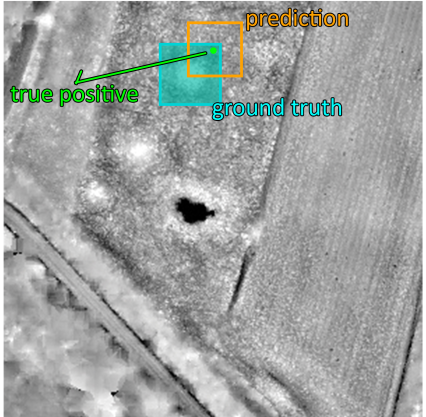
\includegraphics[height=8cm]{images/IOU.png}
\caption{Example of IoU \cite{IOUpaper}}
\end{figure}

Having the APs of all classes, the mAP is then calculated by taking the average of the APs, however in this project separate models were trained for each class, making the AP equal to the mAP.

Another metric is F1, which is given by the following formula:

\begin{equation}
     F1 = 2 * \frac{precision * recall}{precision + recall}
\end{equation}

This metric is especially interesting, when both accuracy and recall are important, enabling an analysis of which is the most favorable confidence value.

Another metric that is also commonly used, is mAP0.5:0.95, the difference with mAP50, is that instead of using only a minimum value of IoU to consider a true positive, several values between 50\% and 95\% are used, with 5\% jumps.

When it comes to lof, training data is unavailable. Additionally, unlike yolo, the original dataset cannot be expanded due to its raw lidar data nature. Given the limited size of the dataset, all the generated .las files were utilized and as mentioned in \cite{lof}, performing inference on training data can yield inaccurate outcomes.

\subsection{Training results}
In this subsection the training results of yolov7 will be shown. Training was performed with all the generated datasets, which are 4 for the tummies and 3 for the hillforts.

As said before the dataset was divided in 85\% for training and 15\% for validation, no test set was used, since the original dataset provided was small, and also because an inference will be made on the LRM images, so it will be possible to analyze the model's performance, analyzing if it found all the annotated objects as well as new ones.

First the training results for the tumuli will be analyzed, and then the results for the hillforts will be analyzed.

In the case of yolov7 training with the original dataset the result was as shown below:

\begin{figure}[H]
    \centering
    {{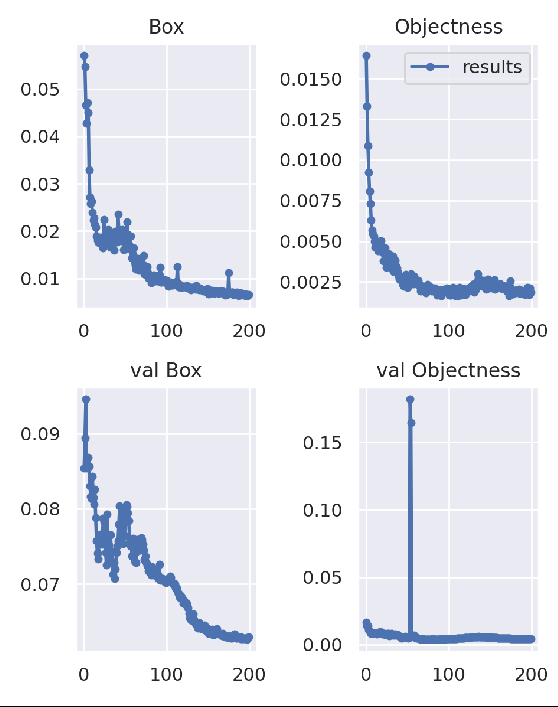
\includegraphics[width=5cm]{images/training/mamoas/notaug1.png} }}
    \qquad
    {{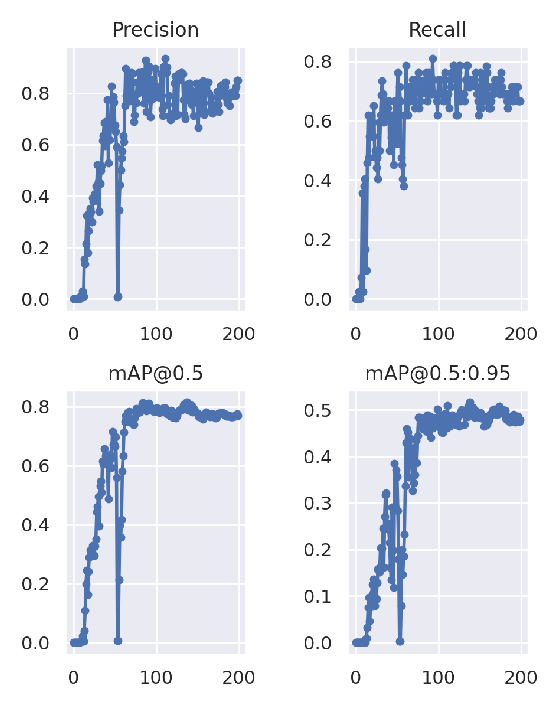
\includegraphics[width=5cm]{images/training/mamoas/notaug2.png} }}
    \caption{Results of Yolov7 training with tumulis non augmented dataset}
    \label{fig:example}
\end{figure}

In the case of training with the dataset augmented with the copy paste algorithm the result was as shown below:

\begin{figure}[H]
    \centering
    {{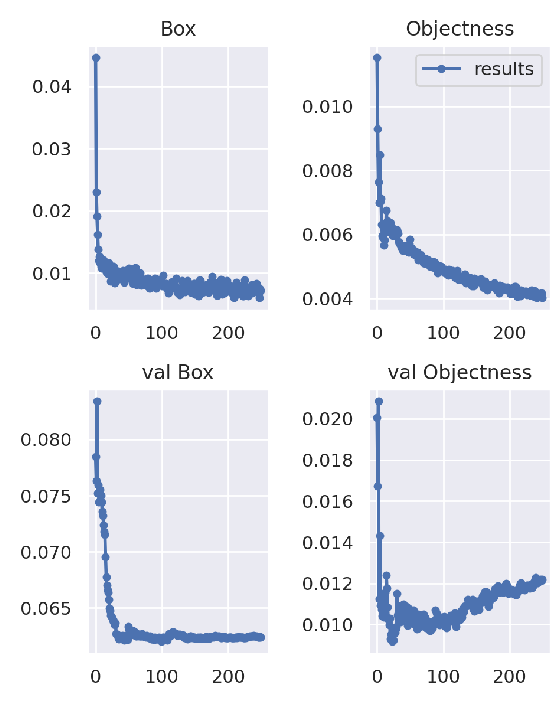
\includegraphics[width=5cm]{images/training/mamoas/aug1.png} }}
    \qquad
  {{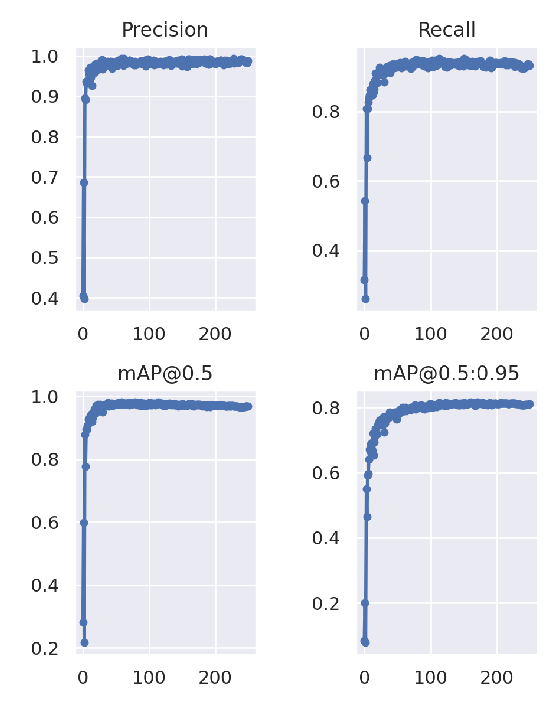
\includegraphics[width=5cm]{images/training/mamoas/aug2.png} }}
    \caption{Results of Yolov7 training with tumulis augmented dataset (copy paste)}
    \label{fig:example}
\end{figure}

In the case of training with the dataset augmented with the simple algorithm the result was as shown below:

\begin{figure}[H]
    \centering
    {{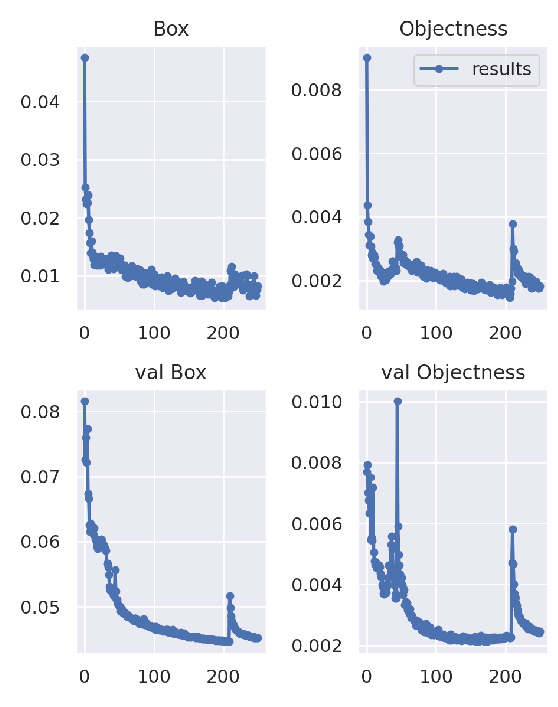
\includegraphics[width=5cm]{images/training/mamoas/maia1.png} }}
    \qquad
    {{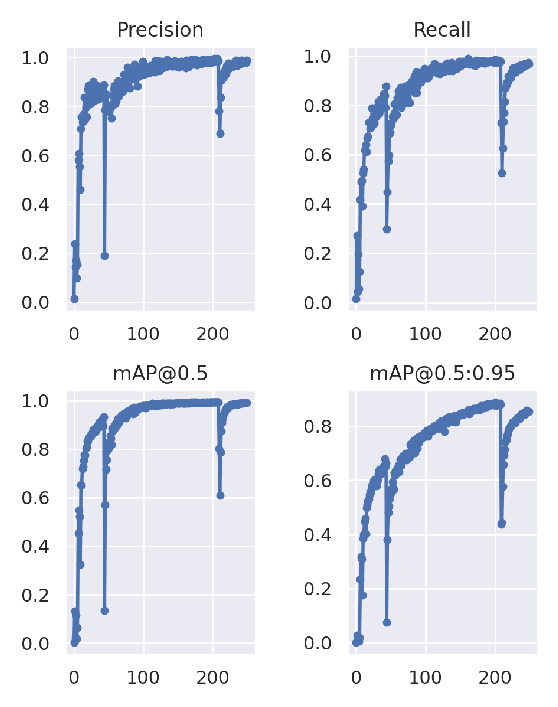
\includegraphics[width=5cm]{images/training/mamoas/maia2.png} }}
    \caption{Results of Yolov7 training with tumulis augmented dataset (simple)}
    \label{fig:example}
\end{figure}

In order to analyze these results, my focus will be solely on the mAP0.5 metric rather than the F1 score. The reason behind this choice is that mAP provides a consolidated value that combines both precision and recall for each epoch, while F1 score represents a graph for each epoch, making it a more complex metric to work with.

As can be observed, in neither of the three models did overfitting occur, including training with the dataset not augmented, which is the most prone to overfitting. It is interesting to note that in the copy paste dataset, after a few seasons, the model stabilized and got very close to 1.

Falta agora para o cross validation!!!!!!
Isso sera uma tarefa nao para o Leonardo de hoje mas sim para o Leonardo do futuro!

In the case of hillforts, the results are as follows:

\begin{figure}[H]
    \centering
    {{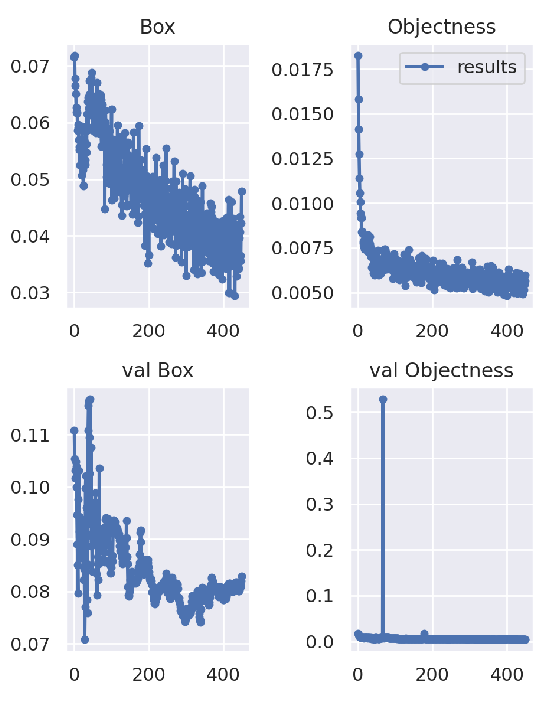
\includegraphics[width=5cm]{images/training/castros/notaug1.png} }}
    \qquad
    {{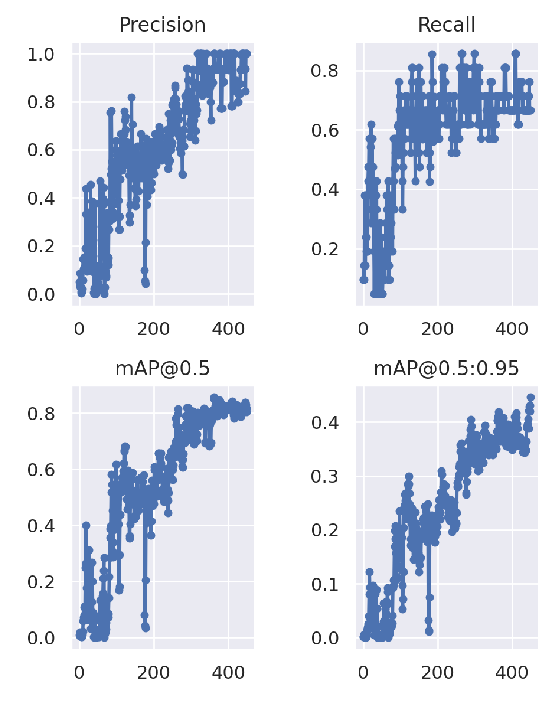
\includegraphics[width=5cm]{images/training/castros/notaug2.png} }}
    \caption{Results of Yolov7 training with hillforts non augmented dataset}
    \label{fig:example}
\end{figure}

In the case of training with the dataset augmented with the copy paste algorithm the result was as shown below:

\begin{figure}[H]
    \centering
    {{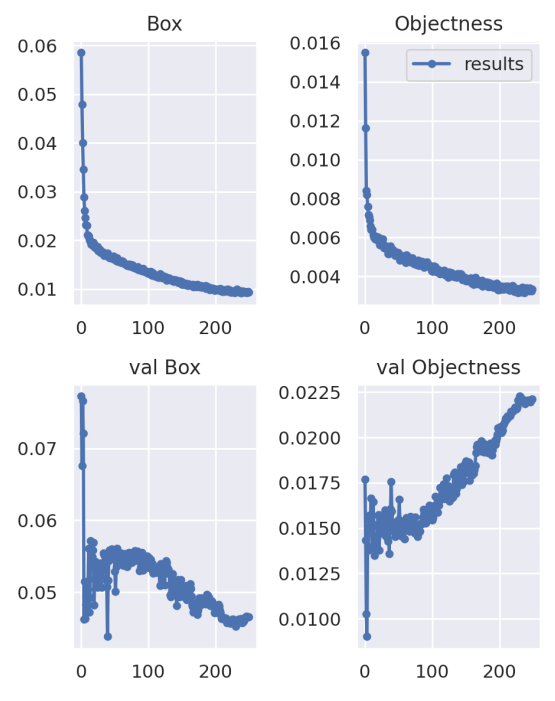
\includegraphics[width=5cm]{images/training/castros/aug1.png} }}
    \qquad
  {{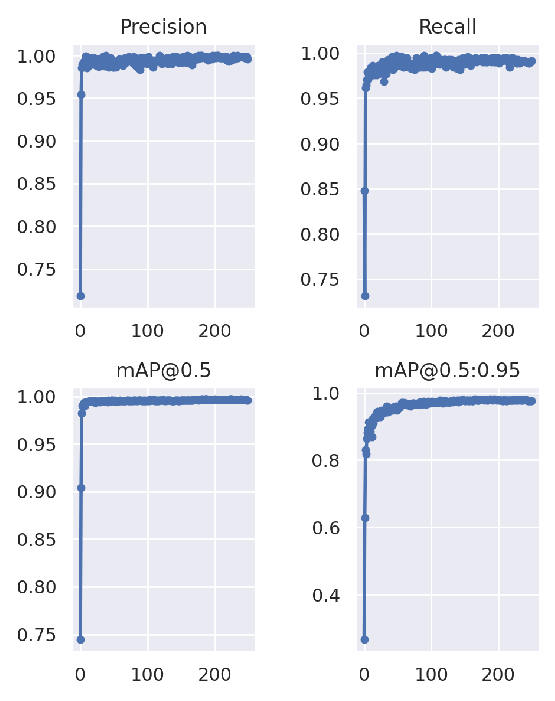
\includegraphics[width=5cm]{images/training/castros/aug2.png} }}
    \caption{Results of Yolov7 training with hillforts augmented dataset (copy paste)}
    \label{fig:example}
\end{figure}

In the case of training with the dataset augmented with the simple algorithm the result was as shown below:

\begin{figure}[H]
    \centering
    {{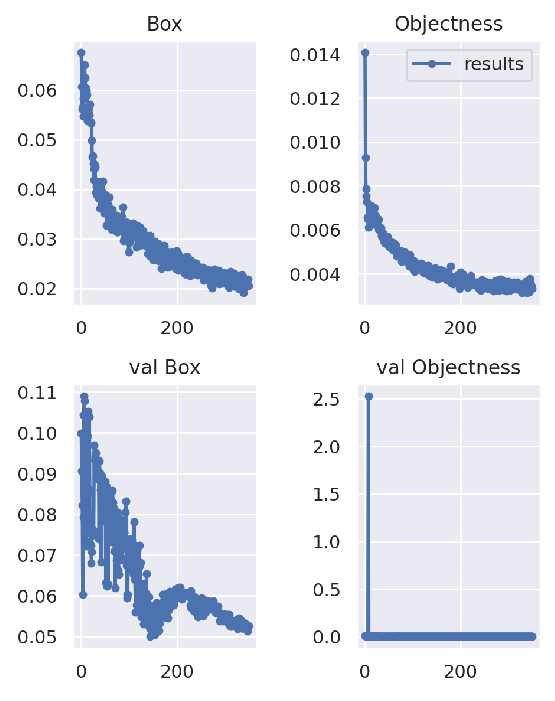
\includegraphics[width=5cm]{images/training/castros/maia1.png} }}
    \qquad
    {{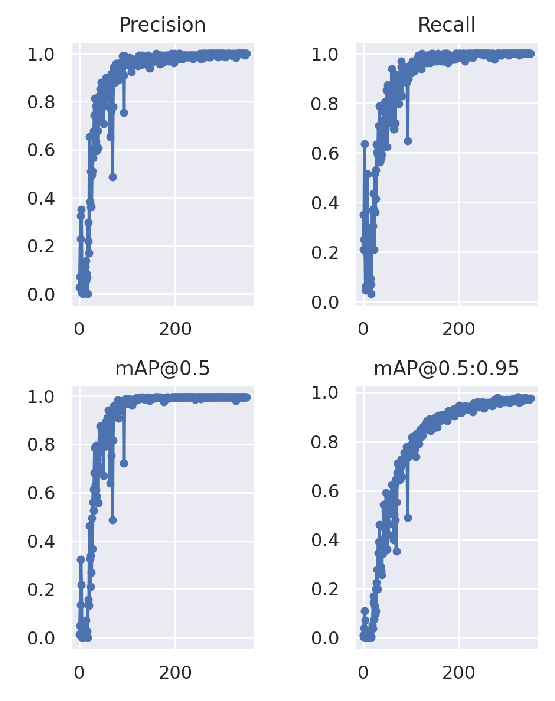
\includegraphics[width=5cm]{images/training/castros/maia2.png} }}
    \caption{Results of Yolov7 training with hillforts augmented dataset (simple)}
    \label{fig:example}
\end{figure}

Similarly to the tummy tucks, in none of the three workouts, overfitting occurred. In the case of the training with the unenhanced dataset, it was necessary to increase the number of seasons in order to make the model converge. And similarly to the tumuli training, the hillforts training with the copy paste dataset, after a few seasons, the mAP was already close to 1.

\subsection{Inference}
In this subsection we will show how the inference was done on the 4 LRM images.

In order to do the inference, a python script was created, in this script, the image is loaded with the PIL library and then, the geographic coordinates of the 4 corners of the image are obtained using the rasterio library, this is possible because the tif images can contain additional information such as geographic coordinates. 

Having the coordinates, and the images being too large to make inferences, an interactive window was used, in order to perform 640x640 pixel crops, however this approach leads to a problem, the crop can be done on top of an object, leaving a part of the object in one image and another part in the next image, to work around this a sliding window was used instead of a fixed window, with the sliding window instead of cropping in a fixed way at each position, the image is scrolled in a systematic way by moving the window pixel by pixel or at a defined interval. This approach allows each object or region of the image to be covered by multiple inference windows, thus avoiding the problem of having parts of an object split between different crops.

When using the sliding window, the image is divided into overlapping windows that move along the image. Each sliding window captures a specific region of the image and then inference is applied to that region individually. As the window slides, new regions are processed, ensuring that all objects or regions are covered.

For the tumuli a 50\% slide was used, because they are small objects, and for the hillforts a 30\% slide was used, because some hillforts occupy almost half of the cropped image.

Once the crop is obtained, it is checked with the aid of a topographic chart to see if the crop contains areas that are likely to have objects. This means that in the crop, there are areas where, for example, there are no houses or roads, thus discarding crops that represent, for example, a residential area in its entirety. After that, inference is performed with YOLO. As mentioned before, YOLO can make multiple detections for the same object, so to overcome this, the NMS function is also used here, discarding overlaps and all inferences with a confidence lower than 25\%. Then, once again, the topographic chart is used to verify if the object is not in an area where it would be impossible to detect.

Once the inference is completed, the identified objects undergo validation using the LOF model. To validate each object, a temporary LAS file is generated. This file is created by utilizing the geographical coordinates of the bounding box. The temporary LAS file is then populated with points that fall within the bounding box. Next, various statistical measures such as mean, median, variance, standard deviation, and covariance are computed using the 14 features extracted from each point. Finally, a prediction is made, returning a value of 1 if the object is determined to be a true positive, or 0 if it is classified as a false negative.

Finally, due to the window slide, for the same object there may be several inferences, because when making the slide the same object may still appear in the next image. To mitigate this, initially the Euclidean distance was used, all the bounding boxes that had the center less than 15 pixels, which corresponds to 7.5 meters on the ground, from another one, would be removed. Initially this approach worked well for the tumuli. However, for the hillforts, a problem occurred, the yolo was detecting hillforts inside larger hillforts, something that does not happen in reality, making it difficult to choose a threshold value for the Euclidean distance. 

In order to get around this, the Euclidean distance was replaced by IoU, as explained before, if the IoU was smaller than a certain value, the smaller hill was discarded, however, the problem still remains, as I checked later in article \cite{IOUpaper}, if the smaller hillfort is fully contained in the larger one and if the area of the smaller one is smaller than the defined threshold value, IoU does not discard, so the problem still remains. So the approach was adopted, instead of being the normal IoU the intersection. Therefore, instead of using the normal IoU, the intersection to be divided by the union, the division of the intersection to be divided by the area of the smallest detection was used. But before that the objects were ordered by area, from the biggest to the smallest, by doing that and using this modified version of the IoU, in the cases where there are detections completely contained inside another, or almost completely contained, they are removed, keeping the biggest one.

In the end, the results are saved in a csv file, containing the geographic coordinates of the bounding box, the confidence given by yolo and the result of the LOF validation.

After the completion of the inference, it is necessary to assess the efficacy of the model by analyzing the detected ground truths and new objects. To facilitate this analysis, a Python script has been developed. Within this script, the ground truth coordinates are loaded and converted into corresponding image pixels, which are further transformed into bounding boxes. Similarly, the coordinates of the objects resulting from the inferences are processed. Utilizing the Shapely library, both the ground truth objects and the inferred objects are converted into polygons. Subsequently, a filtering process is applied to the inference results, removing any inferences with an area smaller than 90\% of the smallest ground truth area. Finally, an interaction is performed on the ground truth objects to determine which inference results intersect with the ground truth.

In the case of inference with the 5 models generated from cross validation, YOLOv7 provides a technique called model ensemble, in which it is allowed to use several models at the same time.

\subsubsection{Model ensemble}
Model ensemble is a technique that consists in using predictions from several deep learning models in order to obtain more robust results than a single model could provide.

By using several models trained on different datasets, in this case the cross validation models, each model generates its own predictions. After that, the predictions are combined, for this, techniques such as majority voting, weighted average, probability average, among others, being possible to make a final decision.

The idea behind this is that each model can capture different features or aspects of the training dataset, and by combining these various models, it is possible to compensate the failures of one model by the successes of others, thus making the result more reliable.

\subsection{LOF model training}
One of the problems encountered earlier in the dissertation was that the inference results contained many false positives, in an attempt to solve this problem, a Local Outlier Model (LOF) was trained on the raw LIDAR data.

Using the .las files generated during creation of the dataset, containing only the points within the bounding box surrounding the object in question, two LOF modelsm, one for tumulis and one for hillforts, were trained using the scikit learn library\cite{lof}.

LOF calculates the local outlier factor for each sample in the data set, taking into account the local density of neighboring samples. It compares the density of the sample against the average density of its nearest neighbors. If the density of the sample is significantly lower than the average density of its neighbors, this indicates that the sample is a possible outlier.

\begin{figure}[H]
\centering
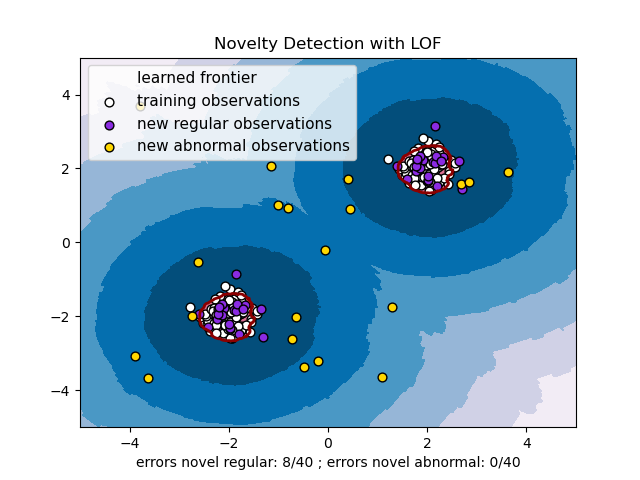
\includegraphics[]{images/lof_example.png}
\caption{Example of clusters generated by LOF}
\end{figure}

In order to train the model, jakteristics library was used, this library allows 14 features to be taken from each point in the point cloud, these features are: eigenvalue sum, omnivariance, eigenentropy, anisotropy, planarity, linearity, PCA1, PCA2, surface variation, sphericity, verticality, nx, ny and nz.

As each point contributed 14 features, this results in a huge amount of features, the mean, median, variance, standard deviation and covariance are calculated, resulting in an amount of 70 features per .las file.

\subsection{Inference results}
In this sub-section it will be showed the results of the inferences made on the 4 LRM images. For this, a script was created, in which the annotations were loaded as well as the results, both the inference results and the annotations were converted to polynomials using the shapely library, then in an interactive way it was checked if any ground truth was intersected by any inference, if so it was accounted for, if there was more than one inference to intersect, only the first one was accounted for as a true positive and all the others as false positives.

Tables will be presented, in which will appear the total number of detected objects, within these objects the number of validations made by the LOF, as well as the true positives, false positives and false negatives, the last 3 are in relation to the total number of detected objects and not to the ones validated by the LOF.

\begin{table}[h!]
\centering
\begin{tabular}{|c c c c c|} 
 \hline
  & Non augmented  & Copy Paste & Simple & Cross Validation(Copy paste) \\ [0.5ex] 
 \hline\hline
 Total & 2324 & 2366 & 1800 & 11446 \\ 
 Validations & 1604 & 1500 & 1354 & 6385 \\
 True positives & 240 & 224 & 210 & 242 \\
 False positives & 2084 & 2142 & 1590 & 11204 \\
 False negatives & 36 & 52 & 66 & 34 \\ [1ex] 
 \hline
\end{tabular}
\caption{Results of inference for tumulis(YOLOv7)}
\end{table}

\begin{table}[H]
\centering
\begin{tabular}{|c c c c|} 
 \hline
  & Non augmented  & Copy Paste & Simple \\ [0.5ex] 
 \hline\hline
 Total & 8002 & 1913 & 5630 \\ 
 Validations & 2799 & 628 & 2145\\
 True positives & 153 & 153 & 113 \\
 False positives & 7849 & 1760 & 5517 \\
 False negatives & 10 & 10 & 50\\ [1ex] 
 \hline
\end{tabular}
\caption{Results of inference for hillforts(YOLOv7)}
\end{table}
It is important to emphasize that the false positives and true positives are relative to the available ground truth, i.e. the training and validation data, and as said before, these data are not the result of an intensive terrain analysis, and there may be among the false positives that are in fact true positives, i.e. new sites discovered by the algorithm that have not yet been annotated.

However, according to the company that provided the data, most of the sites were noted, with only a few missing that may have been missed.

Analyzing the data resulting from the inferences, we can verify that there were many false positives, both in the tumuli and in the castros, however, in the tumuli, the worst case was the one resulting from cross validation, giving about 7 times more false positives than the model resulting from simple augmentation, on the other hand, it was the one that had fewer false negatives, that is, it was the one that managed to detect more ground truth.

In the case of the castros, the model that gave fewer positive false was the one resulting from the copy paste augmentation, giving 1750 negative false and detecting almost all the ground truths, failing only 10 in 163.